\section{\module{noise} ---
         Noise functions}

\declaremodule{extension}{cgkit.noise}
\modulesynopsis{A set of basic noise functions}

\begin{funcdesc}{noise}{x[, y[, z[,t]]]}
Returns a noise value (Perlin) in the range from 0 to 1. The arguments
can be up to 4 floating point values or a sequence with up to 4
floating point values (e.g. a \class{vec3} or a \class{vec4}) with an
optional time value. The return value is a pseudo random number in the
range from 0 to 1. Due to the nature of this noise implementation
(gradient noise) the return value at integer lattice points is always 0.5.

As an example, here is a 2D slice (the grid shows the integer lattice):

\begin{center}
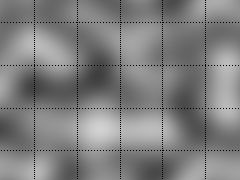
\includegraphics[width=6cm]{pics/noise}
\end{center}

\note{The actual function call depends on the number of arguments, so
calling noise(x,y) is not the same as calling noise(x,y,0). The former
case is a true 2D noise whereas the latter is 3D. The same difference
exists between 3D and 4D.}
\end{funcdesc}

\begin{funcdesc}{snoise}{x[, y[, z[,t]]]}
Returns a signed noise value (Perlin) in the range from -1 to 1. A
call to \code{snoise(args)} is equivalent to \code{2*noise(args)-1}.
\end{funcdesc}

\begin{funcdesc}{pnoise}{point[, t], period[, tperiod]}
Periodic noise function. Basically this is the same as
\function{noise()} but with a periodic return value: \function{pnoise(point)} =
\function{pnoise(point+period)}. The time value can be either part of the point
or it can be specified separately. The point and period must always
have the same dimension. The return value is in the range from 0 to 1.
\end{funcdesc}

\begin{funcdesc}{spnoise}{point[, t], period[, tperiod]}
Signed periodic noise function. The return value is in the range from
-1 to 1. A call to \code{spnoise(args)} is equivalent to 
\code{2*pnoise(args)-1}.
\end{funcdesc}

\begin{funcdesc}{cellnoise}{x[, y[, z[,t]]]}
Returns a pseudo random number which is constant between integer
lattice points. The return value is in the range from 0 to 1.

As an example, here is a 2D slice (the grid shows the integer lattice):

\begin{center}
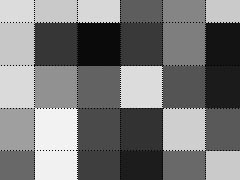
\includegraphics[width=6cm]{pics/cellnoise}
\end{center}
\end{funcdesc}

\begin{funcdesc}{scellnoise}{x[, y[, z[,t]]]}
Signed cell noise. The return value is in the range from -1 to 1. A
call to \code{scellnoise(args)} is equivalent to \code{2*cellnoise(args)-1}.
\end{funcdesc}

\begin{funcdesc}{fBm}{point, octaves, lacunarity=2.0, gain=0.5}
Fractional Brownian motion. The argument point must be a sequence of
either 2 or 3 float values (e.g. a \class{vec3}). This function is a sum of
noise values with different frequencies and amplitudes and is
equivalent to the following code:

\begin{verbatim}
sum = 0.0
amp = 1.0
for i in range(octaves):
    sum += amp*snoise(point)
    amp *= gain
    point *= lacunarity
\end{verbatim}

The return value is in the range from 0 to 1.

As an example, here is a 2D slice (the grid shows the integer lattice):

\begin{center}
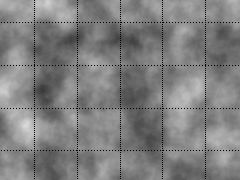
\includegraphics[width=6cm]{pics/fbm}
\end{center}
\end{funcdesc}

\begin{funcdesc}{turbulence}{point, octaves, lacunarity=2.0, gain=0.5}
The code of the turbulence function is very similar to \function{fBm()}. The
difference is that it sums up \code{abs(snoise())} instead of \code{noise()}. 
However, the return value is in the range from 0 to 1.

As an example, here is a 2D slice (the grid shows the integer lattice):

\begin{center}
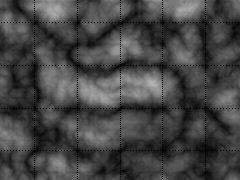
\includegraphics[width=6cm]{pics/turbulence}
\end{center}
\end{funcdesc}


All of the above functions have a vector version that take the same
input parameters but return a vector as result. The output always has
the same dimension than the input. If the time value is specified
separately it does not count to the dimension. For example a call to
\code{vnoise((x,y,z))} returns a \class{vec3}, just as a call to
\code{vnoise((x,y,z),t)}. However, a call to \code{vnoise((x,y,z,t))} 
returns a \class{vec4}.

\begin{funcdesc}{vnoise}{x[, y[, z[,t]]]}
See \function{noise()}.
\end{funcdesc}

\begin{funcdesc}{vsnoise}{x[, y[, z[,t]]]}
See \function{snoise()}.
\end{funcdesc}

\begin{funcdesc}{vpnoise}{point[, t], period[, tperiod]}
See \function{pnoise()}.
\end{funcdesc}

\begin{funcdesc}{vspnoise}{point[, t], period[, tperiod]}
See \function{spnoise()}.
\end{funcdesc}

\begin{funcdesc}{vcellnoise}{x[, y[, z[,t]]]}
See \function{cellnoise()}.
\end{funcdesc}

\begin{funcdesc}{vscellnoise}{x[, y[, z[,t]]]}
See \function{scellnoise()}.
\end{funcdesc}

\begin{funcdesc}{vfBm}{point, octaves, lacunarity=2.0, gain=0.5}
See \function{fBm()}.
\end{funcdesc}

\begin{funcdesc}{vturbulence}{point, octaves, lacunarity=2.0, gain=0.5}
See \function{turbulence()}.
\end{funcdesc}
